\subsection{Shadows}\label{sec:shadowsexperiment}

In the Unity3D[ref] engine there are a number of way to light an environment, each way also has its own limitations when calculating shadows in the environment. Following will be experimentation and analysis of these lighting method will be carried out, to figure out which method is most useful for our use case. 


Directional lighting method uses a orthographic projection from the light source position and direction of the scene, whereas the two other methods uses at perspective projection with a full 360 degree field of view for point but a variable projection angle for spotlight within the range 0[<angle<]180. For the most realistic lighting where the lighting is coming from a single center point, the perspective projections are preferred\cite{unitylighttypes}.

The shadows are compiled as shadow maps as described by \cite{Wimmer2004}.

\begin{figure}
\centering
\begin{subfigure}[t]{0.33\textwidth}
\centering
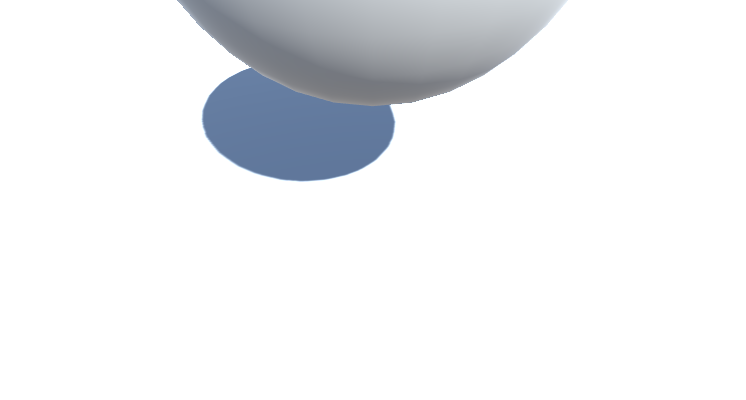
\includegraphics[width=\linewidth]{figures/shadows/directional-cleaned}
\caption{directional}
\label{fig:directional}
\end{subfigure}%
    \hfill
\begin{subfigure}[t]{0.33\textwidth}
\centering
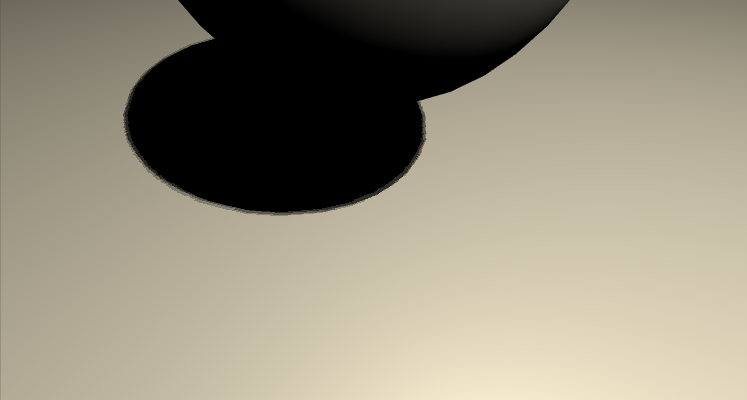
\includegraphics[width=\linewidth]{figures/shadows/point-cleaned}
\caption{point}
\label{fig:point}
\end{subfigure}%
    \hfill
\begin{subfigure}[t]{0.33\textwidth}
\centering

\includegraphics[width=\linewidth]{figures/shadows/point-far-cleaned}
\caption{point far}
\label{fig:point-far}
\end{subfigure}%

\caption{
%(a) directional
%(b) point
%(c) point far
%.
The two other types of lighting in \cite{unitylighttypes}, with two variations of point light, (a) point up close to the object casting the shadow and (b) far from the object.
}
\label{fig:rest-analysis}
\end{figure}


\begin{table}
  \centering
  \begin{tabular}{| c | c | c | }
    \hline
    & Close & Far \\ \hline
    Narrow &  \begin{minipage}{.5\textwidth}
            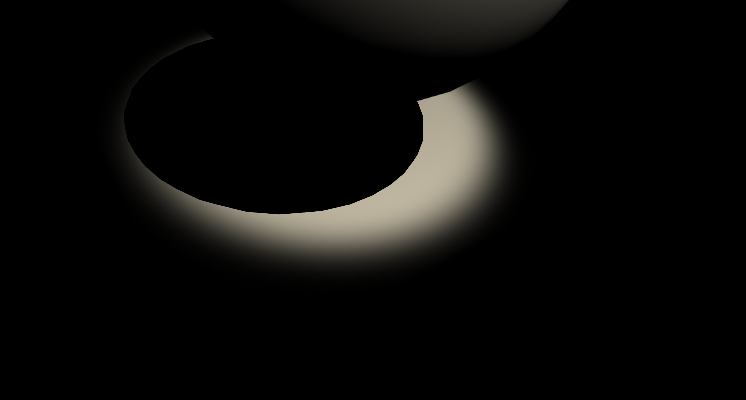
\includegraphics[width=\linewidth]{figures/shadows/spot-cleaned}
            \end{minipage}
            &
            \begin{minipage}{.5\textwidth}
            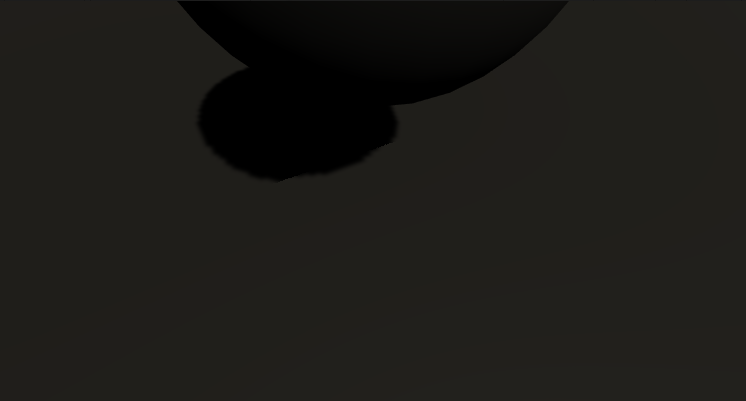
\includegraphics[width=\linewidth]{figures/shadows/spot-far-cleaned}
            \end{minipage}
    \\ \hline
    Wide &  \begin{minipage}{.5\textwidth}
            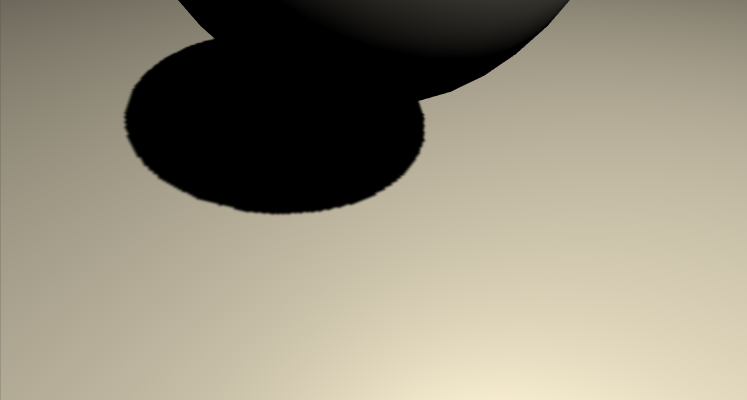
\includegraphics[width=\linewidth]{figures/shadows/spot-wide-cleaned}
            \end{minipage}
            &
            \begin{minipage}{.5\textwidth}
            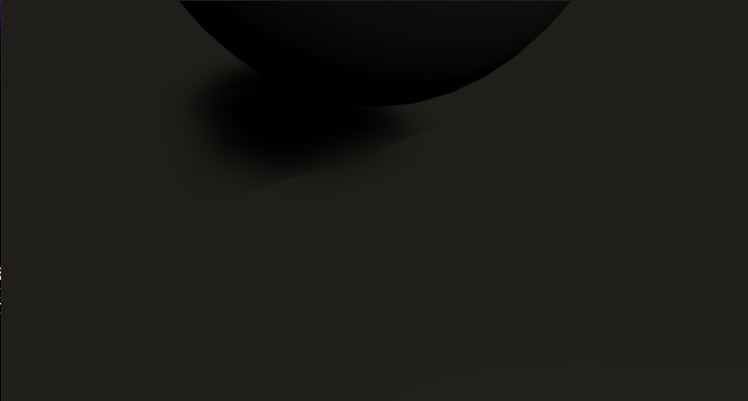
\includegraphics[width=\linewidth]{figures/shadows/spot-wide-far-cleaned}
            \end{minipage}
    \\ \hline
    Widest &  
            \begin{minipage}{.5\textwidth}
            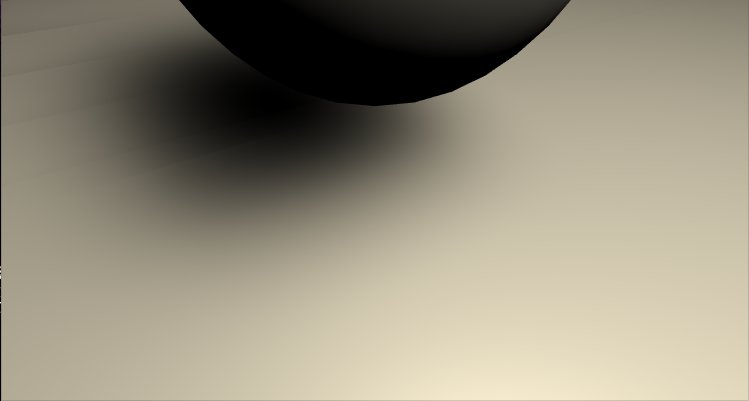
\includegraphics[width=\linewidth]{figures/shadows/spot-widest-cleaned}
            \end{minipage}
            &
            \begin{minipage}{.5\textwidth}
            
\includegraphics[width=\linewidth]{figures/shadows/spot-widest-far-cleaned}
            \end{minipage}
    \\ \hline
  \end{tabular}
  \caption{Spot light analysis}\label{tbl:spot-analysis}
\end{table}


The differing amount pixelation between the types of lighting method is explained by the individual methods varying maximum shadow map sizes\cite{unityshadowmapsize}.